\documentclass[a4paper,12pt]{article}

\usepackage{graphicx}

\setlength{\oddsidemargin}{0in}
\setlength{\textwidth}{\paperwidth}
\addtolength{\textwidth}{-2in}
\setlength{\marginparwidth}{.7in}

\setlength{\headheight}{0in}
\setlength{\headsep}{0in}
\setlength{\textheight}{\paperheight}
\addtolength{\textheight}{-2in}
\setlength{\topmargin}{0in}

\let\olddospecials=\dospecials
\def\dospecials{\samepage \olddospecials}

\setlength{\parindent}{0em}
\setlength{\parskip}{2ex}
\renewcommand{\baselinestretch}{1.5}

\newcounter{note}
\newcommand{\note}[1]{\textbf{NOTE \thenote\addtocounter{note}1: #1}}

\newcommand{\years}{\textrm{y}}
\newcommand{\months}{\textrm{m}}

\newcommand{\rmd}{\textrm{d}}

\newcommand{\event}{E}
%\newcommand{\set}[1]{\textsf{#1}}
\newcommand{\set}[1]{#1}
\newcommand{\group}{\set{G}}
\newcommand{\normal}{\mathcal{N}}
\newcommand{\uniform}{\mathcal{U}}

\iffalse
   $Id: PPD.tex,v 1.1 2004/11/26 09:41:04 ucacdxa Exp $
\fi


\begin{document}

\title{Characteristic orders of events in neurodegenerative diseases}

\author{Hubert M. Fonteijn \and Matt J. Clarkson \and Marc Modat \and Jo Barnes \and Manja Lehmann \and Sebastian Ourselin \and Nick C. Fox \and Daniel C. Alexander}

\date{}

\maketitle

\begin{verbatim}
$Revision: 49 $ $Date: 2010-07-15 08:10:07 +0100 (Thu, 15 Jul 2010) $
\end{verbatim}


\section{Introduction}

Diseases generally develop in characteristic changes. Various symptoms manifest, increase or decrease at each stage. Those symptoms may include a decline in the patient's wellbeing and functionality, a deterioration of tissue integretity at the cellular level or an abnormality in the biochemical makeup of the affected tissue. \note{This probably can be phrased much better}. Modelling disease progression is a key aim of medical science. Such models enhance understanding of the disease and provide a basis for staging patients and thus principled optimization of treatment strategies. 

Most disease staging systems rely on clinical symptoms, because they  are easily accessible to medical practitioners. Clinical symptoms are however only indirect markers of the development of the disease at the cellular and biochemical level. Increasingly, however, a wider variety of measurements have become available to medical researchers which probe diseases at these more fundamental levels of disease progression. Such measurements therefore offer exciting opportunities to develop much more precise staging procedures.

Let us for instance consider Alzheimers Disease (AD). The earliest clinical symptom of Alzheimer's Disease (AD) is a decline in episodic memory, which is followed by a more general decline in cognitive abilities, a deterioration of mood and the gradual loss of bodily functions. The cellular hallmark of AD, on the other hand, is the appearance of extracellular Amyloid placques and intracellular neurofibrillary tangles (NFTs). Braak and Braak \cite{braak1991neuropathological} describe the development of AD using the pattern in which NFT's spread through the brain. They show that initially, NFT's appear in the entorhinal cortex, at which stage patients do not experience any overt symptoms. After this initial phase, the NFT's spread to the hippocampus and other medial temporal lobe structures, which marks the onset of the decline in episodic memory. In a later stage, association cortices in the parietal and prefrontal cortex are affected. The NFT's affect the primary cortices only in the very last stages of the disease. A third hallmark of AD is the loss of neuronal tissue, which is also called neuronal atrophy. The local appearance of amyloid placques and and NFT's are thought to be the key factors causing neuronal atrophy, although the mechanism through which this occurs is still under debate \cite{van2007current}. Interestingly, there is now ample evidence that neuronal atrophy can be detected using Magnetic Resonance Imaging \cite{baron2001vivo, du2007different, fox1996visualisation, jack1997medial, lerch2005focal, thompson2001cortical} \note{TO DRC: Are these appropriate references?} and that MRI can therefore be used to follow disease progression \emph{in vivo}. Both studies from Thompson et al. \cite{thompson2003dynamics} and Scahill et al. \cite{scahill2002mapping} show that the development of neuronal atrophy indeed follows a similar pattern as the appearance of NFT's: patients with mild symptoms show only atrophy of the hippocampus and other memory-related areas, whereas in later stages other parietal and prefrontal areas are affected.

Currently, there are two staging procedures available for AD patients. Clinical tests, such as the Mini-Mental Stage Exam (MMSE), classify patients into a Mild Cognitive Impairment stage, when they show only abnormal episodic memory performance, or in a mild or moderate AD stage, when they show more severe cognitive deficits. These tests show however limited specificity with respect to the development of AD at the cellular level. Braak and Braak \cite{braak1991neuropathological} on the other hand, provide a very detailed staging paradigm based on how NFT's spread through the brain. This paradigm is however based on post mortem data and can therefore not be used for clinical assessments. MRI scans, on the other hand, are relatively easy to obtain in vivo and would therefore be much better placed to base a cellular classification procedure on. Dubois et al. \cite{dubois2007research}	indeed propose to include MRI as a marker for probable AD, although they do not propose any further subdivision. Current methods therefore do not fully exploit the potential of MRI to provide detailed models of disease progression.

This has motivated us to develop a novel model that can reconstruct disease progression patterns from data sets that characterize the symptoms of patients in a range of disease stages. Crucially, the model does not require \emph{a priori} staging of the patients, but instead it provides a novel classification framework, which ranks patients along the order of events. The critical assumption behind our model is that the occurrence of symptoms occurs in an order which is largely consistent between patients.  Our model describes disease progression as a series of events. Each event is defined as the \emph{onset} of a symptom, i.e. the moment at which a symptom becomes detectable. In the context of AD, events could include for instance the onset of significant atrophy in a region, or deviation of episodic memory performance from the performance of healthy age-matched controls. We model disease progression by reconstructing the most likely chain of events from the data. Although in this study, we apply this model to MRI data of neurodegenerative diseases, we stress its applicability is much wider than neurodegenerative diseases alone and that we can estimate the model from any measurements that reveal the presence of absence of any kind of symptom.  

Our model is fitted in two stages: In the first stage we estimate the precedence matrix, which quantifies the probability of any event preceding any other event. In the second stage, the precedence matrix is used to reconstruct the most likely ordering of events. We can estimate the precedence matrix both using longitudinal and cross-sectional data. In the presence of longitudinal data which fully cover the disease progression in each patient, the precedence matrix is straightforward to define for each patient. This type of data is however rarely available. Cross-sectional data on the other hand are much more practical to acquire, but only provide a snapshot of disease progression for each subject. In this study, we develop a simple procedure to derive the precedence matrix for cross-sectional data. Another advantageous feature of our model is the ease with which different kinds of events can be fused. This will in the future facilitate the fusion of different data types into one single model for disease progression.

We demonstrate the method here using MRI and clinical data from familial Alzheimer's Disease and Huntington's Disease. Familial AD (fAD) is a rare inherited variant of AD which causes early onset of AD symptoms. Because fAD mutation carriers are at high risk to develop AD, it is feasible to enroll them in studies before they develop any clinical symptoms, thereby providing a unique opportunity to study cellular or biochemical symptoms in the very earliest stages of AD. \note{In the event that the HD data produce nice results, add some more background info on HD}. 

We use regional atrophy data from both patients and healthy age-matched controls to determine when regional atrophy significantly deviates from atrophy in healthy subjects. We then reconstruct disease progression models and show good agreement with existing knowledge about disease progression in AD and HD, but at a much finer level of detail. Further the models uniquely place key clinical events within the chain of atrophy events for the first time, which demonstrates nicely the ability of the new technique to combine different kinds of events int he progression model.

\section{Theory}
\label{theory}
We model disease progression as a series of events. Each examination of a patient provides a snapshot of their progression in which some events have ocurred and others have not. Measurements during the exam provide an estimate of the probability of each event. Here we use binary probabilities: if evidence for an event is signifcant then p(E) = 1, otherwise p(E) = 0. Figure \ref{FigureConceptual} illustrates the reconstruction of the order of events which consists of three steps: determining the likelihood that each event has occurred in each measurement, estimating the precedence matrix and calculating the ordering of events that best explains the precedence matrix. The precedence matrix P contains in each entries $P_{i, j}$ the probability $p(\event_A\prec\event_B)$ that event $E_i$ precedes event $E_j$.  We define $\set{X}_{A\prec B}$ as the set of subjects in which we observe event A but not event B and thus the probability that $E_i$ precedes $E_j$:

\begin{equation}
\label{drpsum}
p(\event_i\prec\event_j) = \frac{|\set{X}_{A\prec B}|}{|\set{X}_{A\prec B}| + |\set{X}_{B\prec A}|}
\end{equation}

\begin{figure}
\centering
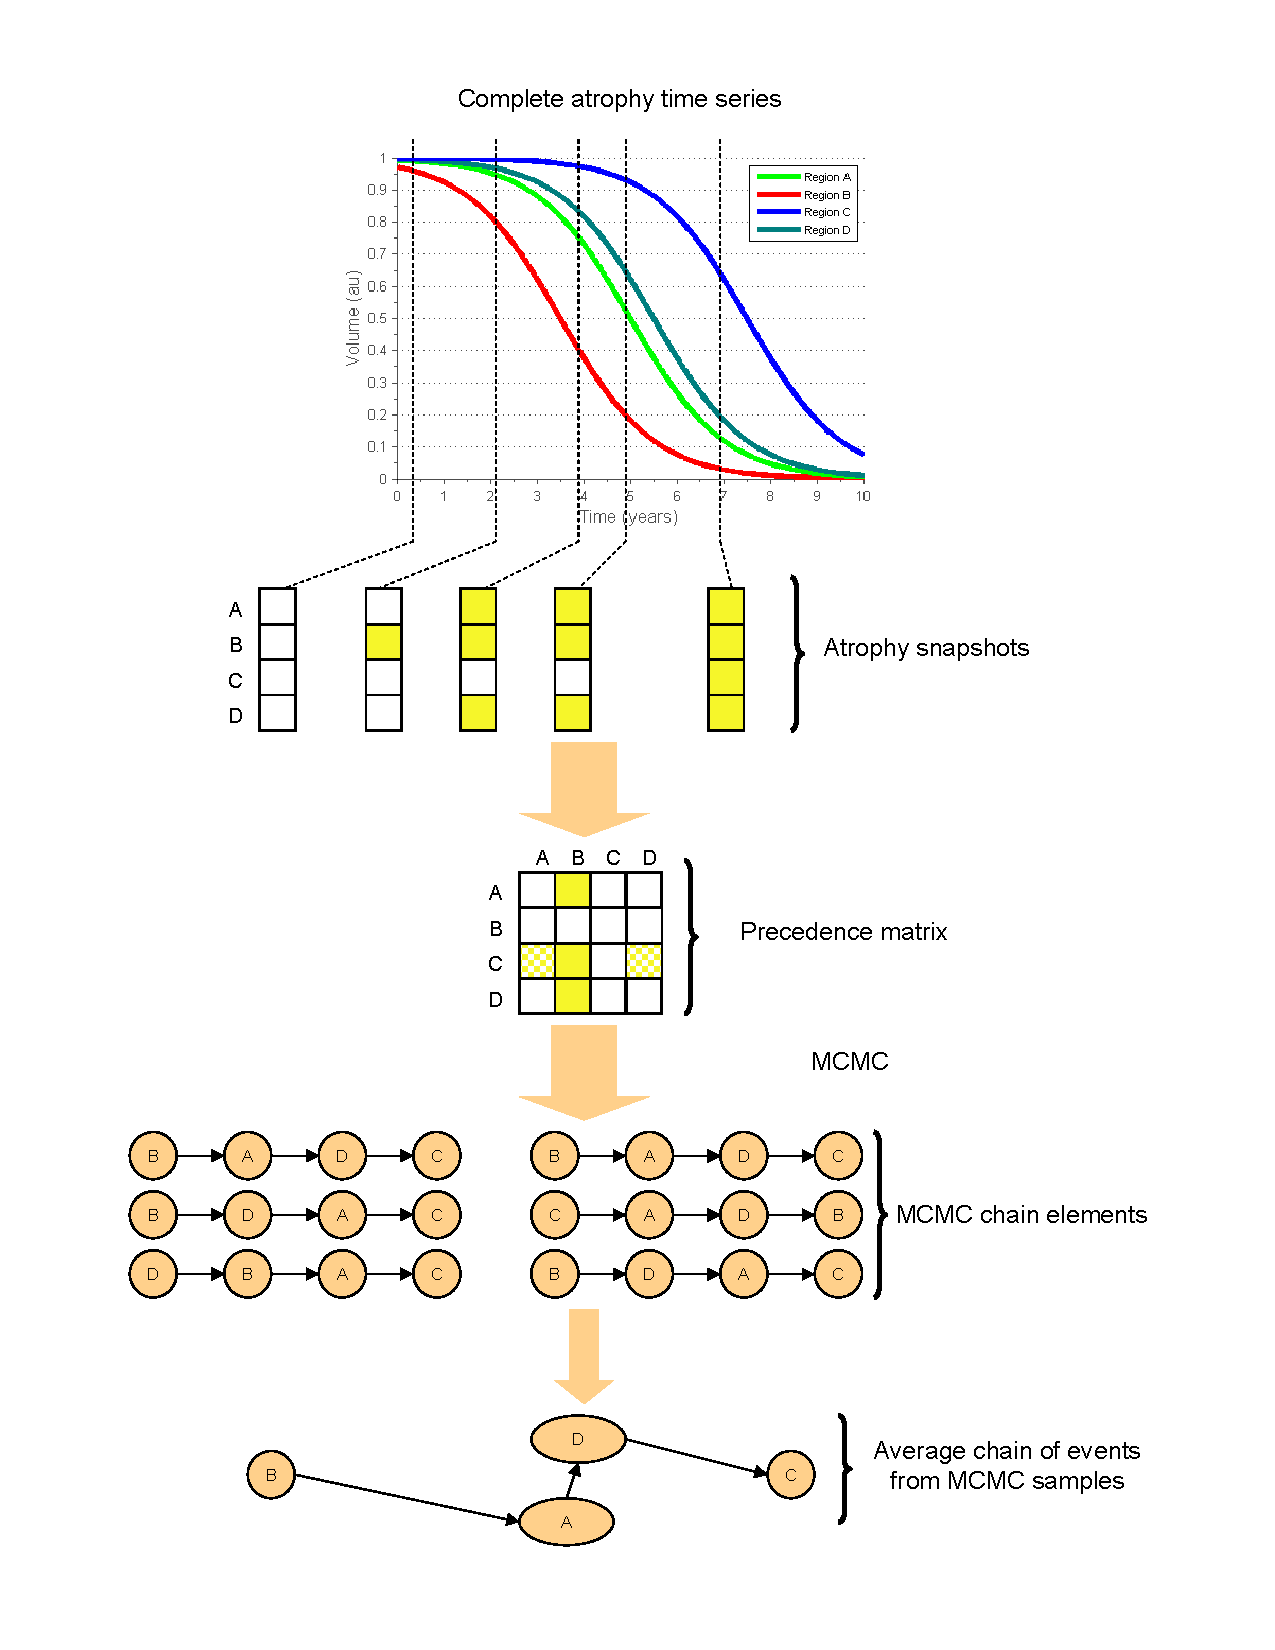
\includegraphics[width=120mm]{figures/FigureConceptual}
\caption{Conceptual overview of the disease progression model. The upper panel shows the full atrophy patterns of four regions. The data represent snapshots of these patterns, from which a precedence matrix is derived. This precedence matrix is then used in the MCMC procedure to reconstruct the order of events. The atrophy patterns of region A and D are temporally almost indistinguishable. This causes intermediate values in the precedence matrix for the probability that atrophy in region A precedes atrophy in region D. This in turn results in frequent switching in the positions of A and D in the MCMC procedure. This can be summarized by the mean and standard deviation of the positions of each region, which is shown in the lowest panel. The horizontal position indicates the average position of each event (which is almost equal for region A and D), while the width of the ellipses indicate the standard deviation (which is much higher for region A and D than for other regions. We introduce differences in the vertical position of atrophy events only to clarify visualization.}
\label{FigureConceptual}
\end{figure}

in which $|.|$ denotes the cardinality of the set. 

We use a MCMC algorithm \cite{gilks1996markov} to sample from the posterior distribution on the event orderings.  The starting point $k_0$ is a random ordering of the events. The likelihood of an order of events  $\event_{k(1)}\prec\event_{k(2)}\prec\cdots\prec\event_{k(N)}$ comes directly from P:  

\begin{equation}\label{seqmodlik}
L(k) = \prod_{i=1}^{N-1}\left(\prod_{j=i+1}^N p(\event_{k(i)} \prec \event_{k(j)}) \right).
\end{equation}

A perturbation $k'$ of the current model swaps the positions of two randomly chosen events.  The next step $k_1 = k'$ with probability $\min(a, 1)$ where $a = L(k')/L(k_0)$ is the likelihood ratio; otherwise $k_1 = k_0$.  Repeating the procedure produces the MCMC chain. 

Each element in the MCMC chain contains one event ordering. Our final step computes the mean and standard deviation of the poterior distribution on the position of each event. We plot each event at its mean position to viesualize the degree of certainty of each part of the estimated ordering. The bottom panel of figure \ref{FigureConceptual} for example shows low conficence in the relative positions of events A and D, because the time courses of both events are almost indistinguishable. The positions of events A and D are thus interchangeable in the MCMC chain, which results in a very similar mean position for both events. We further characterize the uncertainty around the mean position of an event by calculating its standard deviation from the MCMC chain, which we visualize with the width of the events' icon.

\section{Methods}
In this study we use clinical symptoms and the onset of regional atrophy as measured by MRI as events in our disease progression study. Section \ref{data_acquisition} provides information about the demographics of the AD and HD data sets and the MRI scanning parameters that were used. Section \ref{preprocessing} explains the preprocessing pipeline that we used to derive regional atrophy estimates from the MRI images. Section \ref{model_estimation} concludes by reviewing the details of estimating the disease progression model in the case of this particular data set.

\subsection{Data acquisition}
\label{data_acquisition}
\subsubsection{familial Alzheimer's Disease data}
The fAD data we use has been previously analyzed in Ridha et al. \cite{ridha2006tracking}. Briefly, nine carriers of autosomal mutations associated to Alzheimer's Disease were recruited from the Cognitive Disorders Clinic at the National Hospital for Neurology and Neurosurgery. 25 Age-matched and sex-matched controls (two to three controls per mutation carrier) were also recruited from spouses, relatives and healthy volunteers. All participants gave written informed consent as
approved by the local ethics committee. All mutation carriers underwent comprehensive clinical and neuropsychological assessments, including the mini-mental state examination (MMSE) and volumetric MRI scans, at each visit (41 visits: three to eight per patient). Each control patient had two MRI scans (except two participants who had four scans each) adding up to 54 scans in total. The clinical status of each mutation carrier was classified at each time
point as: 1) familial Alzheimer�s disease, if the patient fulfilled National Institute of Neurological and Communicative Disorders and Stroke and Alzheimer�s Disease and Related Disorders (NINCDS-ADRDA) diagnostic criteria for probable Alzheimer�s disease; 2) MCI, if the patient fulfilled MCI criteria;13 and 3) presymptomatic, if participants fell short of both NINCDS-ADRDA and MCI criteria. All mutation carriers became affected and so have a known date of onset, except one who has remained presymptomatic. In this case, the age of onset was estimated from the mean age of onset from other affected members in the participant�s pedigree. We refer to Ridha et al. for a more detailed description of this data set.

Imaging was undertaken with two scanners: in the period between 1991 and 2000 a 1.5 T GE Signa MRI scanner (General Electric Medical Systems, Waukesha, WI, USA) was used. T1 images were acquired using a Spoiled Gradient Echo technique with the following parameters: (256 x 128 matrix, field of view 24 x 24 cm, TR/TE/NEX/FA=35 ms/5 ms/1/35�) yielding 124 contiguous 1�5 mm thick slices. Between 2000 and 2005 scans were acquired on a different 1.5 T GE Signa scanner. On this scanner T1 images were acquired using an inversion recovery fast spoiled gradient echo sequence with the following parameters: 256 x 256 matrix, field of view 24 x 18 cm, TR/TE/TI/NEX/FA=14 ms/5.4 ms/650 ms/1/15�, yielding 124 contiguous 1.5 mm thick slices.

\subsubsection{Huntington's Disease data}
The HD data have been previously analyzed in Henley et al. \cite{henley2009relationship}. Sixty-one patients with genetically confirmed HD were recruited from the multidisciplinary HD clinic at the National Hospital for Neurology and Neurosurgery, London and the Huntington�s Disease Clinic at Addenbrooke�s Hospital, Cambridge. Forty patients were classified as �early HD� (stages 1 and 2) \cite{shoulson1979huntington}, and 21 patients were gene carriers without motor signs, i.e. premanifest. Twenty neurologically normal controls, either patients� partners or at-risk subjects who had tested negative for the HD gene expansion, were also recruited. All subjects gave written informed consent in accordance with the Declaration of Helsinki, and the study had local research ethics committee and Hospital Trust approval. Subjects underwent assessment by a neurologist and psychologist, using the UHDRS clinical rating scale [Huntington Study Group (1996)] which comprised motor, functional and cognitive assessments. We refer to Henley et al. for a more detailed description of this data set.

Imaging for the HD data set was undertaken using a 1.5 T GE Signa MRI scanner \note{To DRC: Is this true???}. T1 images were acquired using an inversion recovery prepared fast spoiled gradient echo sequence with the following parameters: 256x256 matrix, field of view 24 x 18 cm, TR/TE/TI/NEX/FA = 13 ms/5.2 ms/650 ms/1/13 �, yielding 124 contiguous 1.5 mm thick coronal slices.

\subsection{Preprocessing}
\label{preprocessing}
The preprocessing pipeline consists of two stages: extracting anatomically defined regions and determining voxel-wise atrophy using non-rigid registration methods. The preprocessing pipeline is illustrated in figure \ref{flowchart_preprocessing}.

\begin{figure}
\centering
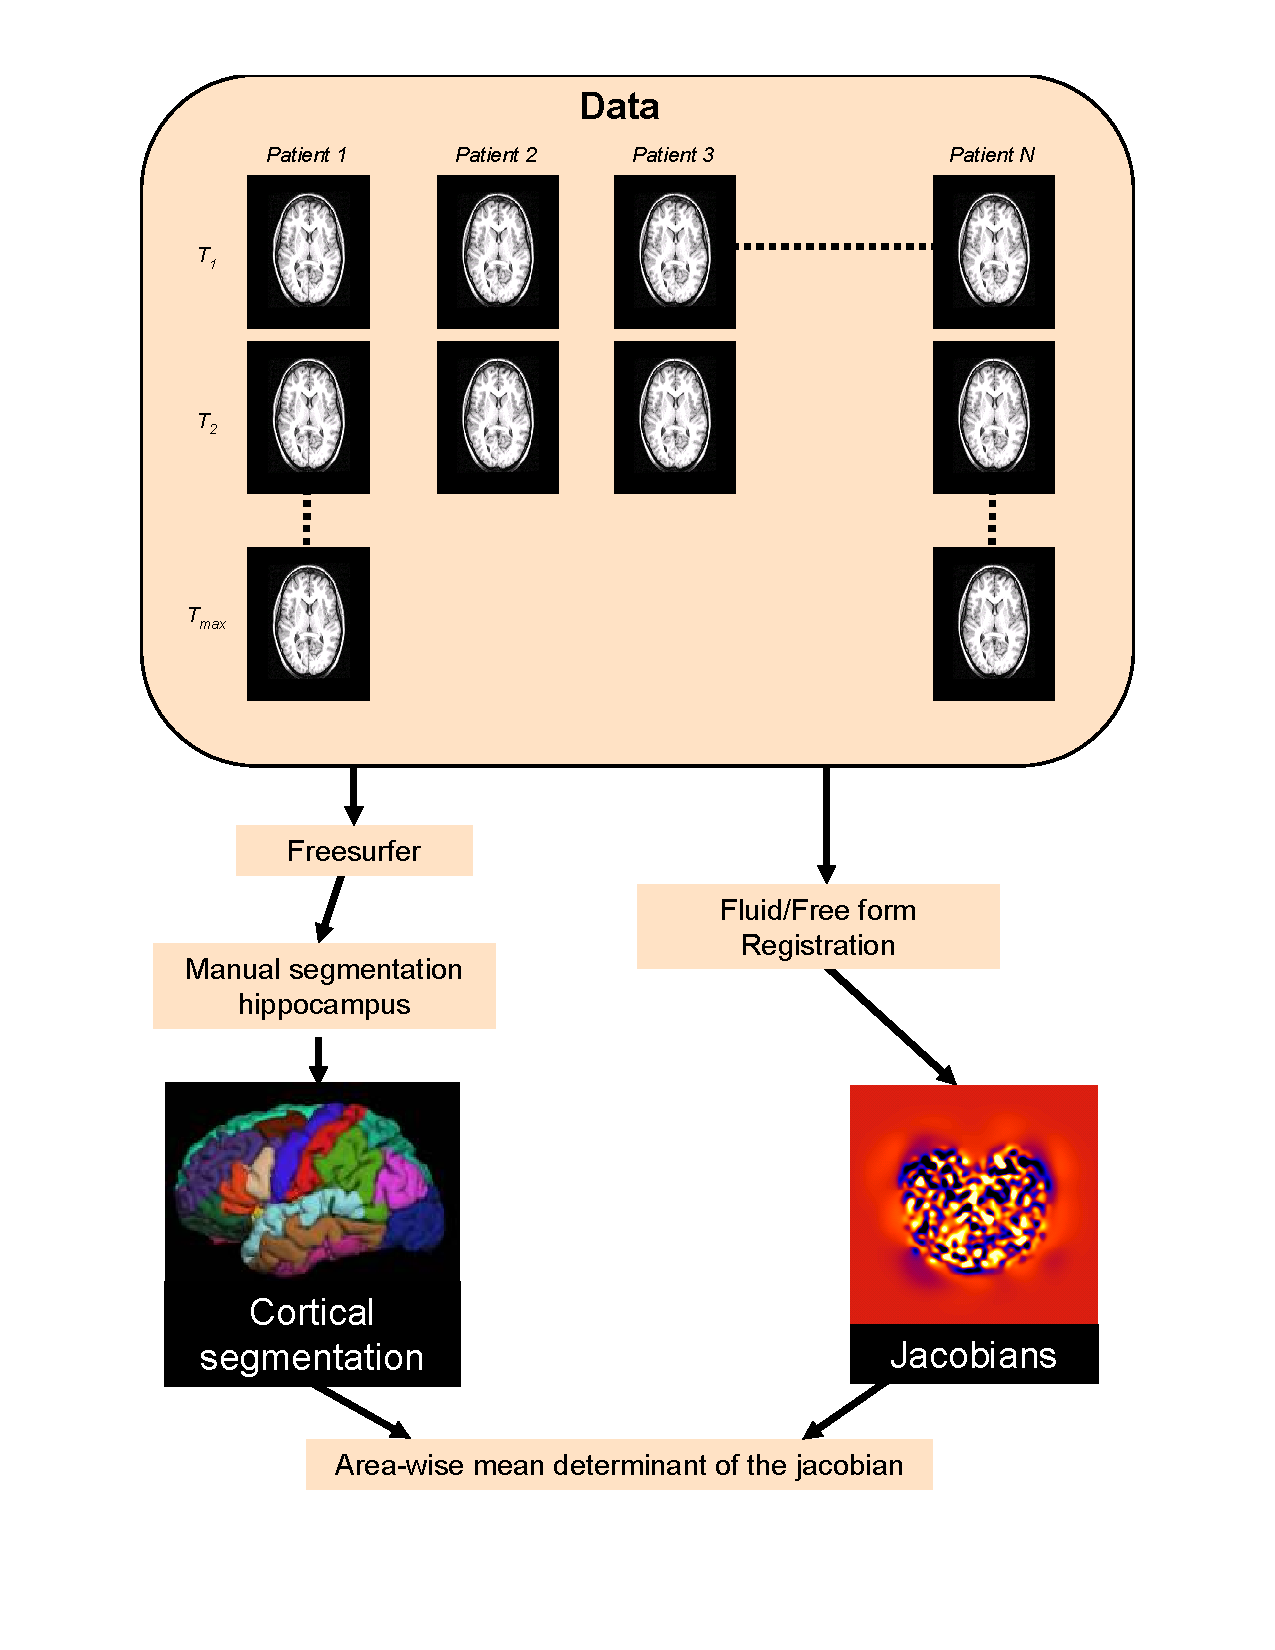
\includegraphics[width=120mm]{figures/flowchart_data}
\caption{Flow chart of the preprocessing pipeline. The T1 images of all subjects are entered in two processing steps: the derivation of anatomically defined regions using freesurfer and the determination of voxel-wise atrophy by using non-rigid registration methods. The determinant of the voxel-wise Jacobians that are the result of this registration procedure are then averaged over all the freesurfer areas.}
\label{flowchart_preprocessing}
\end{figure}

We use freesurfer to segment the brain into cortical and subcortical structures. Freesurfer starts with a grey matter/white matter segmentation. It then uses a labelling procedure on each subject's data which is based on a training set of scans which have been segmented manually \cite{fischl2002whole, fischl2004automatically}. Thus an anatomical segmentation is achieved which is dependent on each subject's individual anatomy and which has been shown to be statistically equivalent to manual segmentation \cite{fischl2002whole}. Freesurfer has however well-documented problems with segmenting subcortical structures, such as the hippocampus. In the fAD data, we therefore supplement freesurfer's segmentation with manually segmented hippocampi in each subject. \note{For DRC: Are these problems well-documented? What reference?} The left and right hippocampus is manually traced by \note{For DRC: whom? couldn't find it in Ridha et al}.

We calculate voxel-wise atrophy values using two non-rigid registration methods and assess whether the disease progression model is robust with respect to the choice of registration method. We use a fluid registration \cite{freeborough1998modeling} and a free form deformation registration \cite{modat2009fast} method. In both methods, a rigid registration is performed first to realign the repeat scans to the baseline scan. Then either a viscous fluid model \cite{freeborough1998modeling} or a set of cubic B-splines \cite{modat2009fast} is used to locally deform the repeat scan to match the baseline scan. In each voxel, the change that is required by this matching procedure is quantified by the determinant of the Jacobian of the deformation field. In the last stage of the preprocessing, we calculate regional atrophy by averaging the logarithm of this Jacobian value over the segmented regions. \note{To DRC: This could probably benefit from some input from Marc/Matt}.

\subsection{Model estimation}
\label{model_estimation}
We require the estimation of the probability for each event that it has occurred in any of the measurements. In the case of the regional atrophy estimates we do this by performing a z-test on the patients' atrophy values in each region against the null hypothesis that they are not significantly different from the regional atrophy in healthy controls. If in a measurement this null hypothesis is rejected in region A, we set p(E) to 1, otherwise we set it to 0. The clinical events \{A, B, C\} reflect transitions between levels of MMSE scores and they therefore do not require hypothesis tests to infer whether they have occurred or not.

The MCMC algorithm is implemented as is outlined in section \ref{theory}, using flat priors on the event orderings. We use 500000 iterations of the MCMC algorithm and discard 5000 as burnin samples. We retain every 50th sample of the remaining iterations, from which we calculate the average position of the regions in the event orderings and their standard deviation.

\section{Experiments}

In this section we review the results of applying the disease progression model to the AD and HD data sets. We show in general good agreement of our model with existing knowledge about disease progression in each disease.

\subsection{Disease progression familial Alzheimer's Disease}
Figure \ref{ADPooledHemispheresPrecMat2FluidRegGoose} shows the key result of estimating the disease progression model using the fAD data. We calculate the regional atrophy using the free-form deformation algorithm, which we then average over hemispheres. Figure \ref{ADPooledHemispheresPrecMat2FluidRegGoose} shows the estimated order of the occurrence of significant regional atrophy. We also include the clinical events and show their place in the order of events. The lower half of figure \ref{ADPooledHemispheresPrecMat2FluidRegGoose} shows snapshots of the order of (atrophy) events projected on a subject's brain. Classification \{A\} is the minimal classification with which patients were entered into the AD category and therefore takes the first place in the event ordering. The progression of atrophy starts in the hippocampus, in the precuneus and the intraparietal cortex and spreads then through other temporal and parietal regions. In later stages more prefrontal areas are affected. The primary motor and sensorimotor cortices are the last ones to be affected. It is of interest to note that classification \{B\} takes a relatively early place in the ordering, after classification \{A\} and atrophy in the intraparietal region and the hippocampus. 

Figure \ref{ADBHPoolFluidRegPrecMat2Order} shows the average position in the events chain of each region. The width of each icon indicates the standard deviation of its position. The icons of consecutive events often show considerable overlap, indicating low confidence in their relative ordering. However even in the densest part of the ordering, events that are four or five positions apart generally show little overlap. Therefore we can have high confidence in the relative ordering of events that are four or more positions apart.

\begin{figure}
\centering
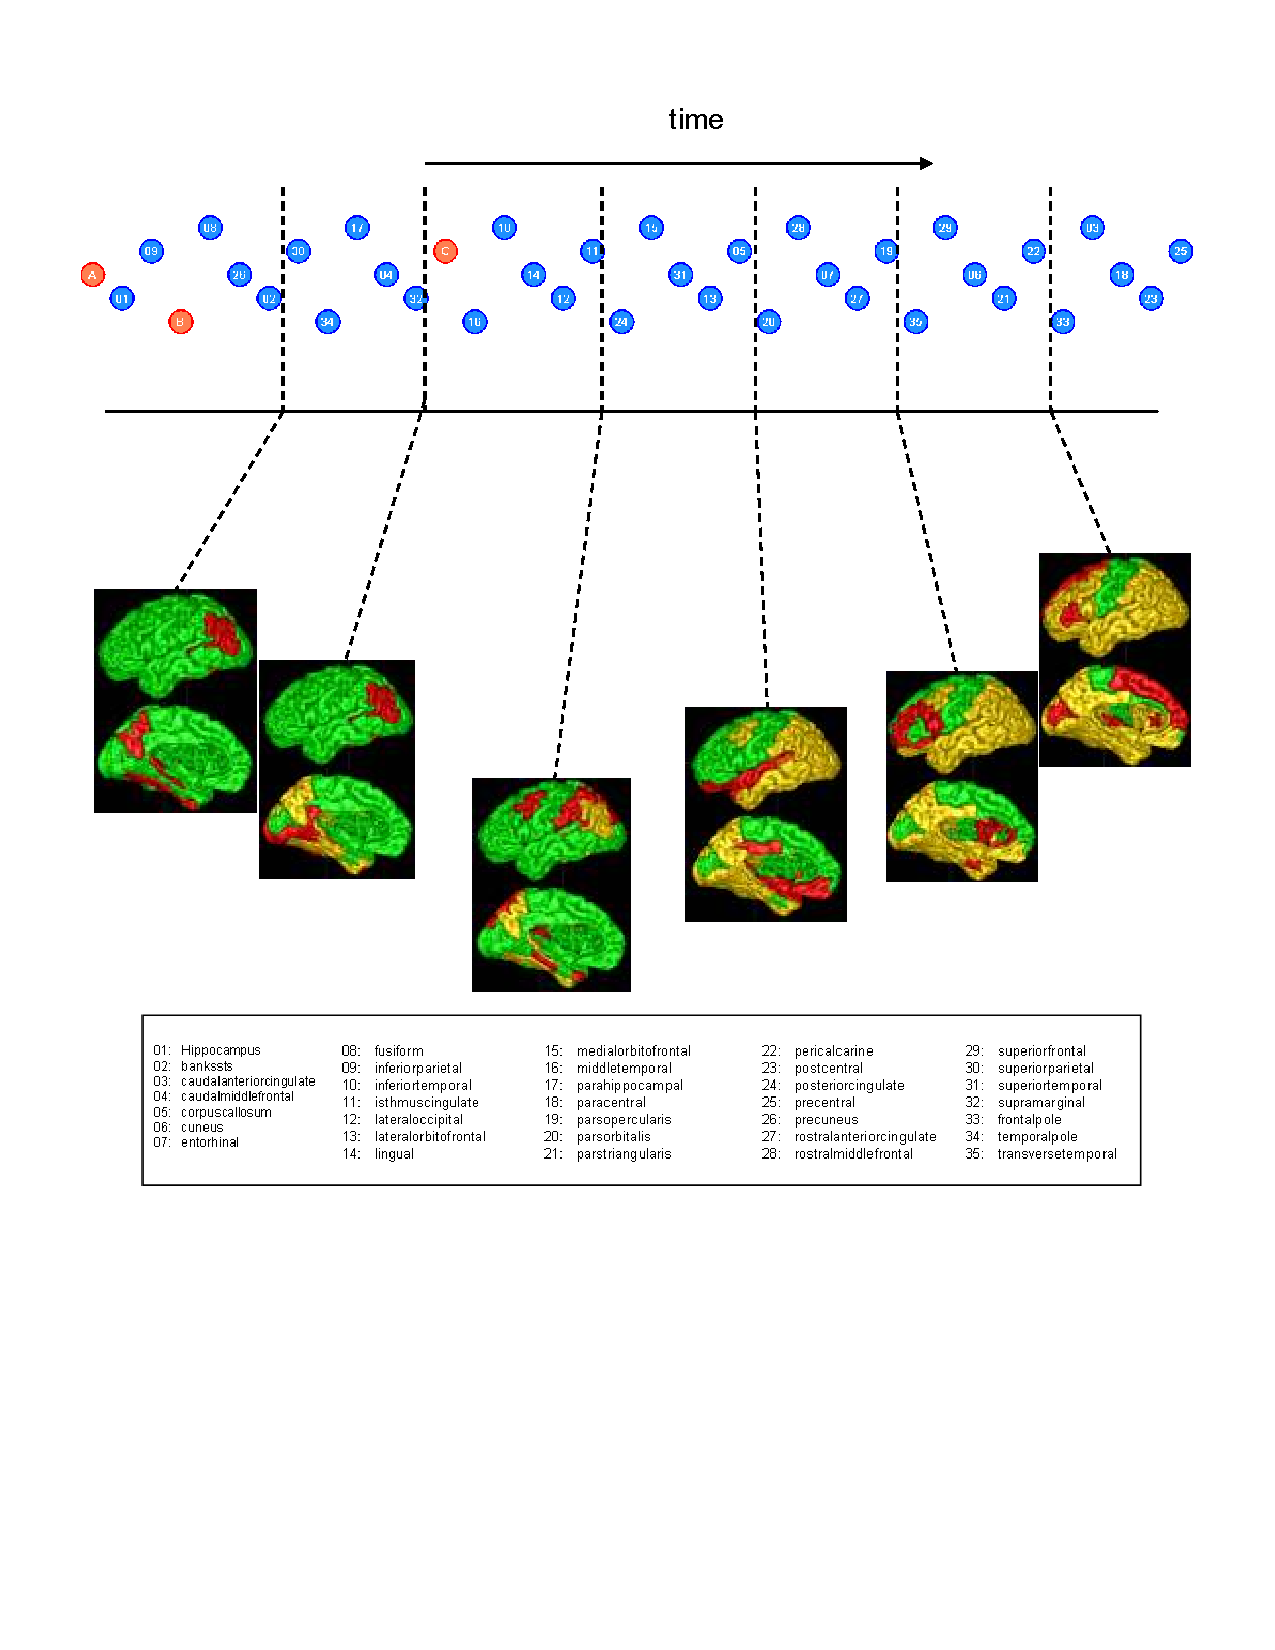
\includegraphics[width=120mm]{figures/ADPooledHemispheresPrecMat2FluidRegGoose}
\caption{Disease progression in fAD. The upper half shows the order in which significant atrophy occurs in all regions. Again, differences in vertical position are only introduced to clarify visualization. The lower half shows snapshots of this pattern of atrophy, projected onto an individual patient's brain.}
\label{ADPooledHemispheresPrecMat2FluidRegGoose}
\end{figure}

\begin{figure}
\centering
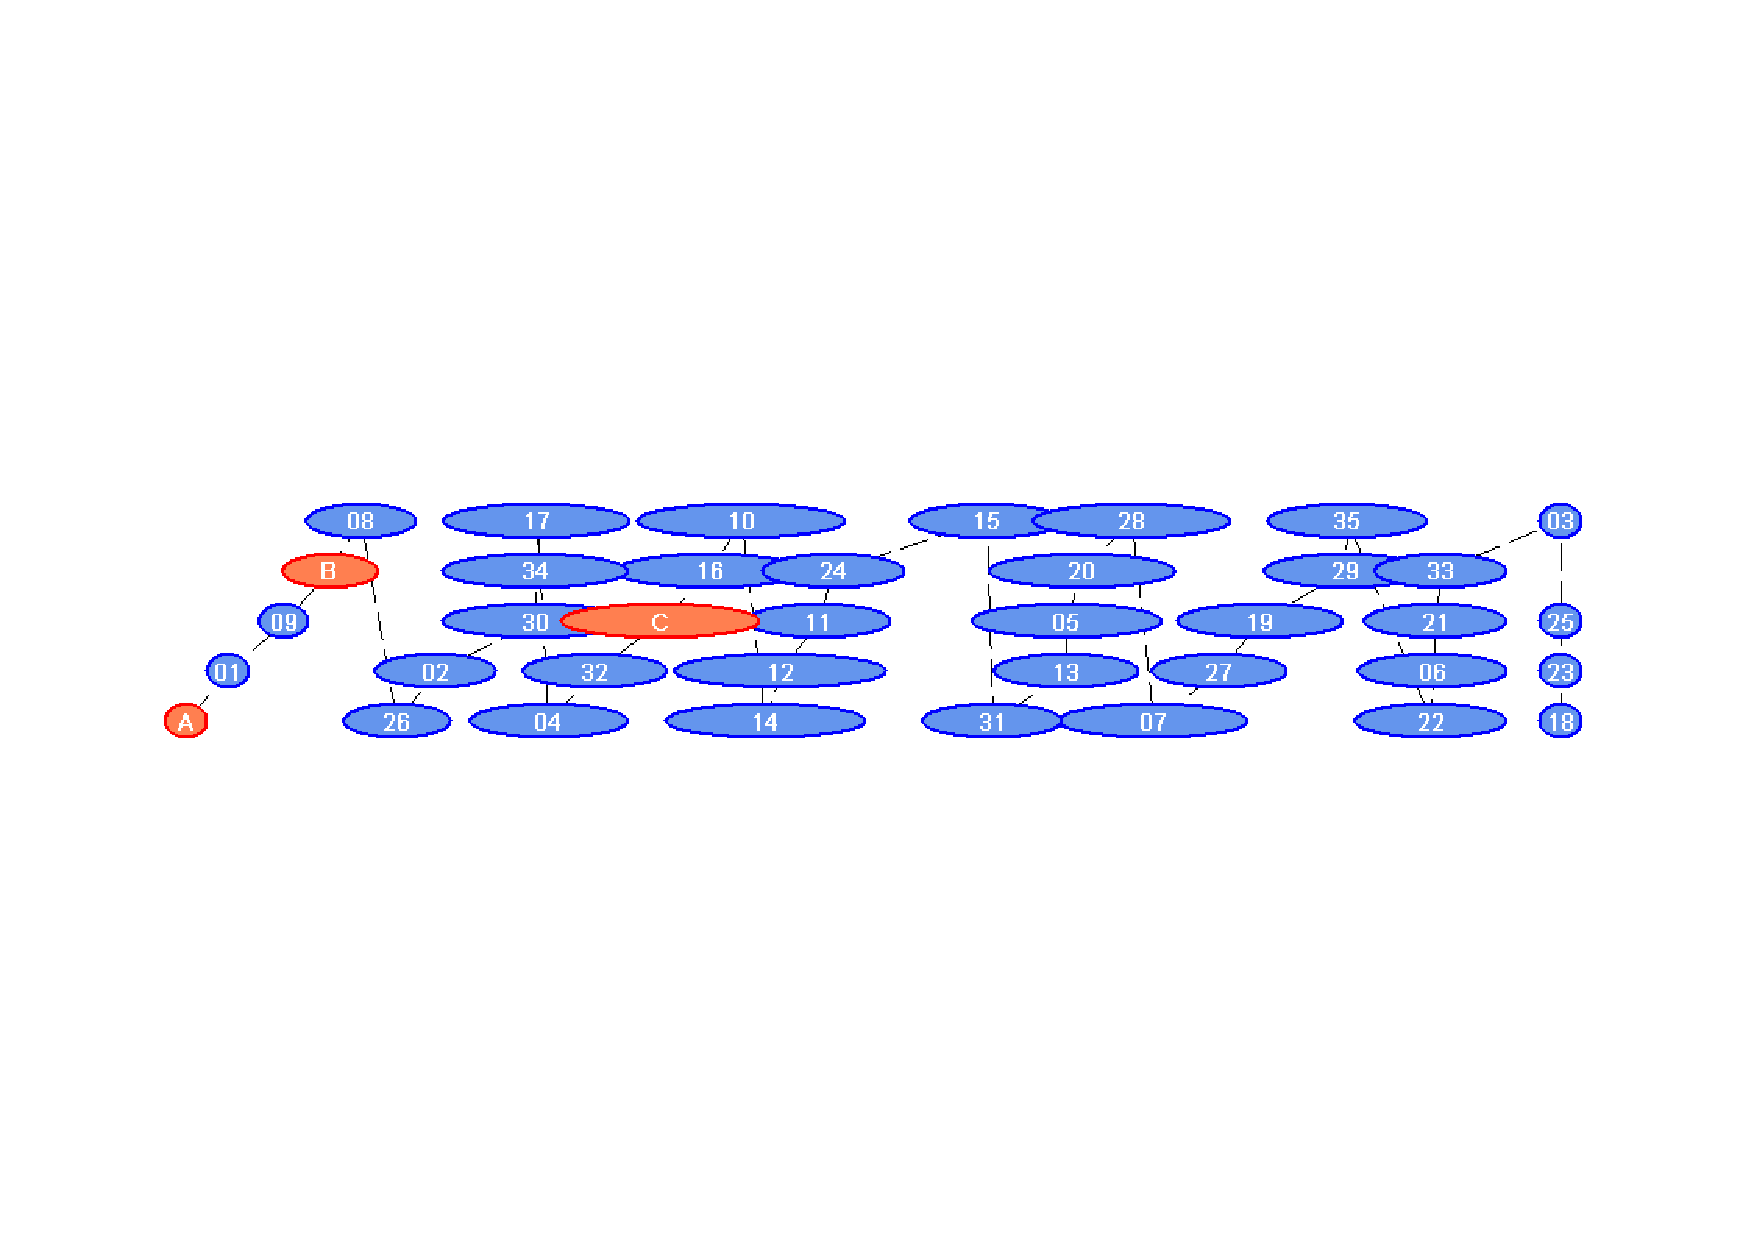
\includegraphics[width=120mm]{figures/ADBHPoolFluidRegPrecMat2Order}
\caption{Average ordering of atrophy events. The average position is indicated in the horizontal position of the centre of the ellipses. The width of the ellipses indicates the standard deviation around the position and is in the same units as the average position.}
\label{ADBHPoolFluidRegPrecMat2Order}
\end{figure}

In the previous experimtent, we have averaged over hemispheres to increase statistical power per region and to increase the ease of interpretation of our results. Now we show consitency between hemispheres in figure \ref{ADFluidRegPrecMat2Hemispheres} shows the results of fitting our disease progression model to data of both hemispheres at the same time, again using the free form deformation method. In this case, the place of each region in the events order is color-coded and spatially mapped onto the surface of a patient's brain. We indeed observe a generally symmetric pattern of disease progression which is in line with the results in figure \ref{ADPooledHemispheresPrecMat2FluidRegGoose}. We conclude that averaging between hemispheres is a valid step. \note{To DRC, there are statistical ways of testing this. I will look into this later}.

\begin{figure}
\centering
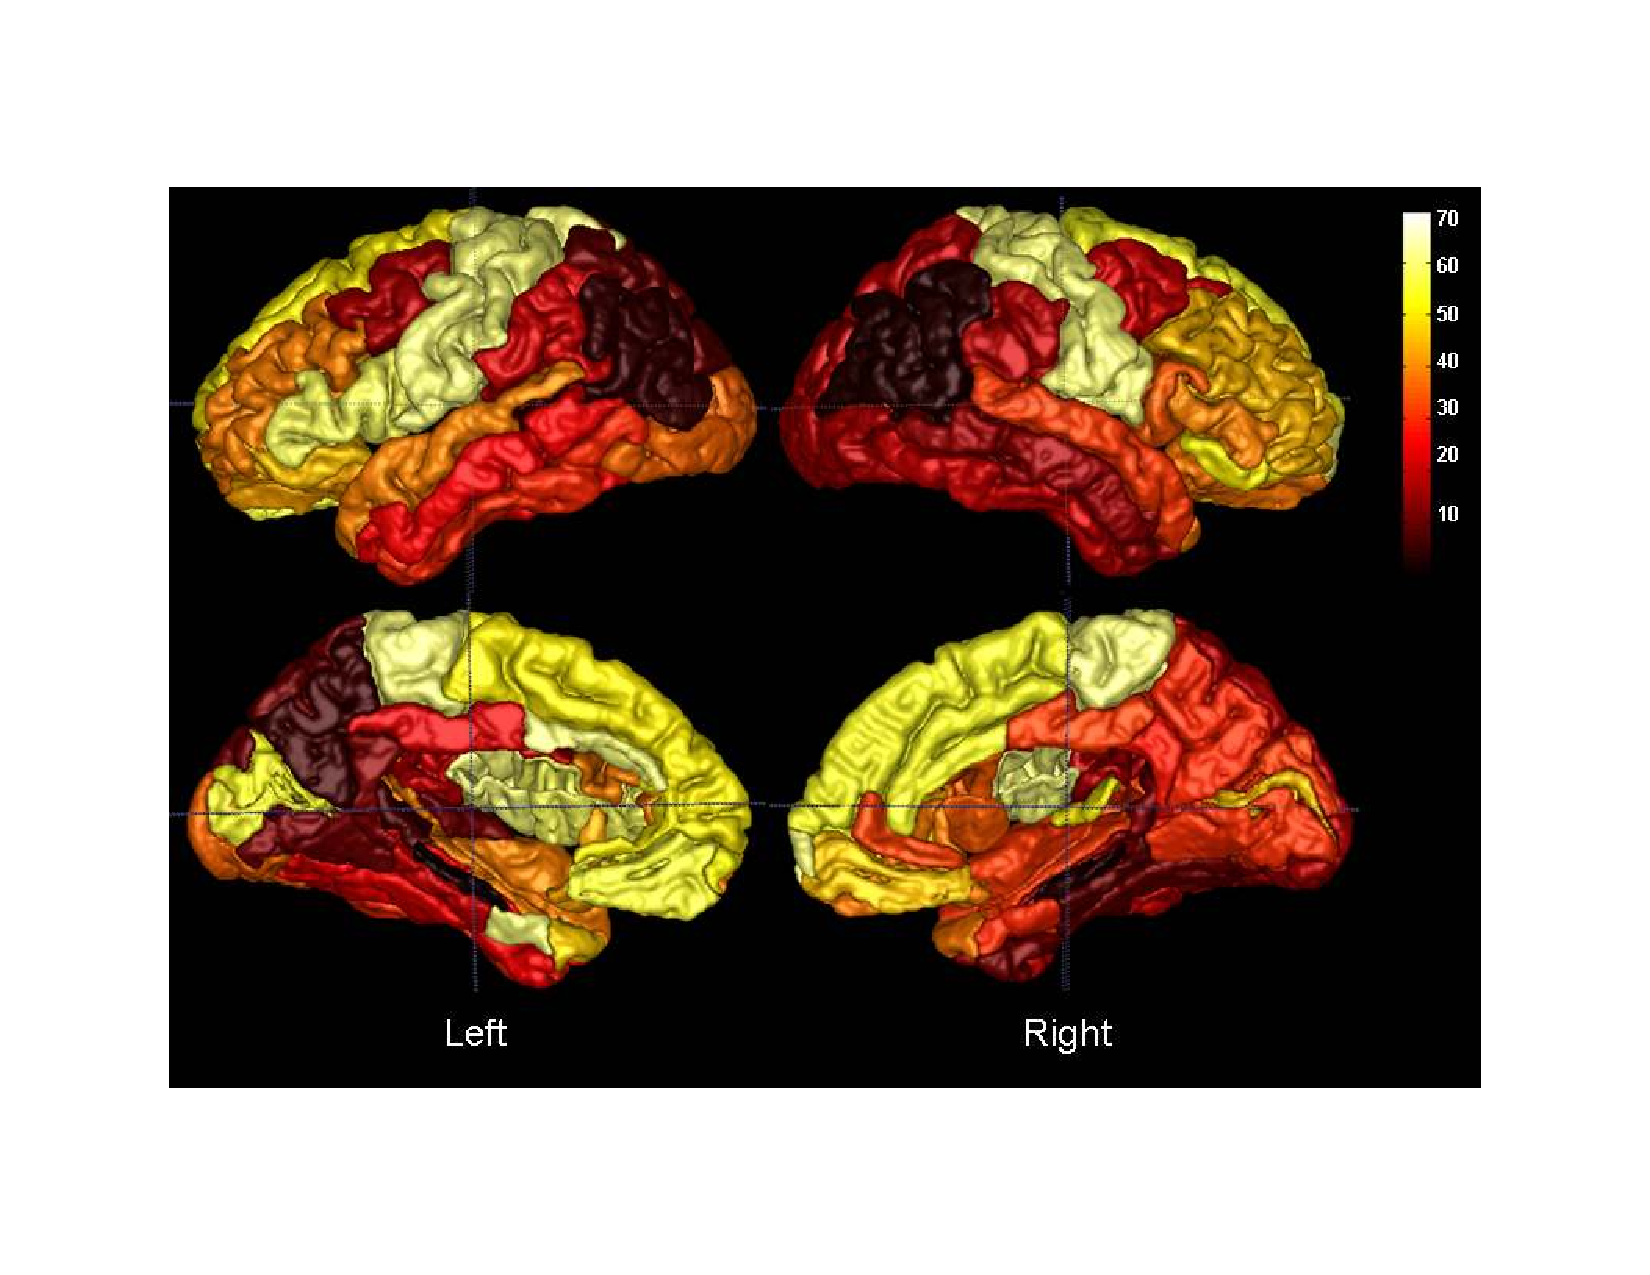
\includegraphics[width=100mm]{figures/ADFluidRegPrecMat2Hemispheres}
\caption{Disease progression in fAD, when fitted in both hemispheres simultaneously (for supplementary material)}
\label{ADFluidRegPrecMat2Hemispheres}
\end{figure}

We hypothesize that the disease progression model is a valid tool for staging patients along the events order. We stage patients in two steps: In the first step, we calculate at each point along the events chain which areas are predicted to show significant atrophy. In the second step, we determine what areas show significant atrophy in each patient and we correlate this with the atrophy patterns of the model. We then classify the patient by determining the point along the chain of events that shows the highest correlation. Figure \ref{ADPooledHemispheresGooseClassify} replicates the results of figure \ref{ADPooledHemispheresPrecMat2FluidRegGoose} but now shows the classification of patients as well. In all cases, the temporal order of time points follows the order of disease progression, although in some cases two different time points are classified as belonging to the same progression stage.

\begin{figure}
\centering
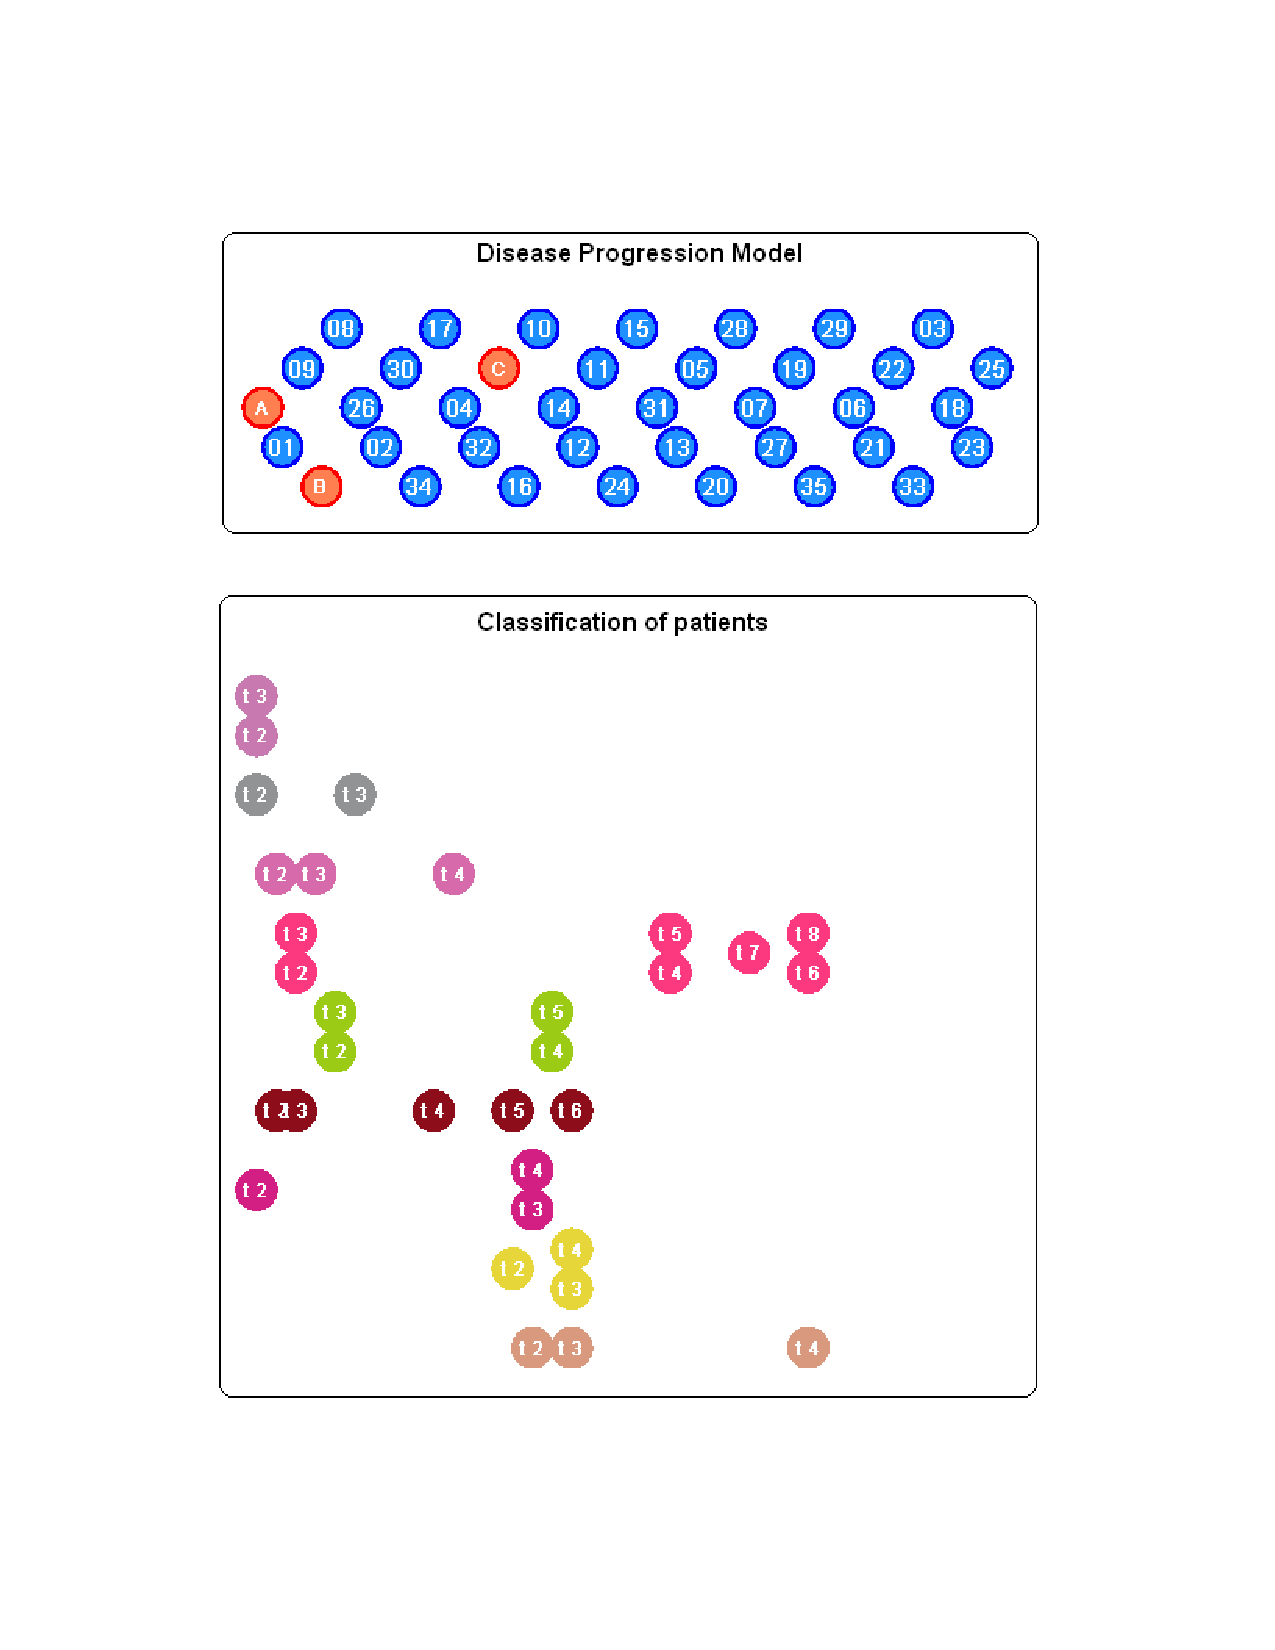
\includegraphics[width=120mm]{figures/ADPooledHemispheresGooseClassify}
\caption{Classification of subjects with the disease progression model. Each subject is indicated by a different colour.}
\label{ADPooledHemispheresGooseClassify}
\end{figure}

The disease progression model should be robust with respect to the choice of registration method. We therefore estimate the model using atrophy measures derived from the fluid registration method and the free form registration method. Figure \ref{ADCompareReg} shows that the results are broadly similar for both methods, although some differences in ordering of the prefrontal areas can be observed. We also investigate the dependence of the disease progression model on the significance level with which we determine significant regional atrophy and show again robustness to this parameter \note{Not yet shown}. 

\begin{figure}
\centering
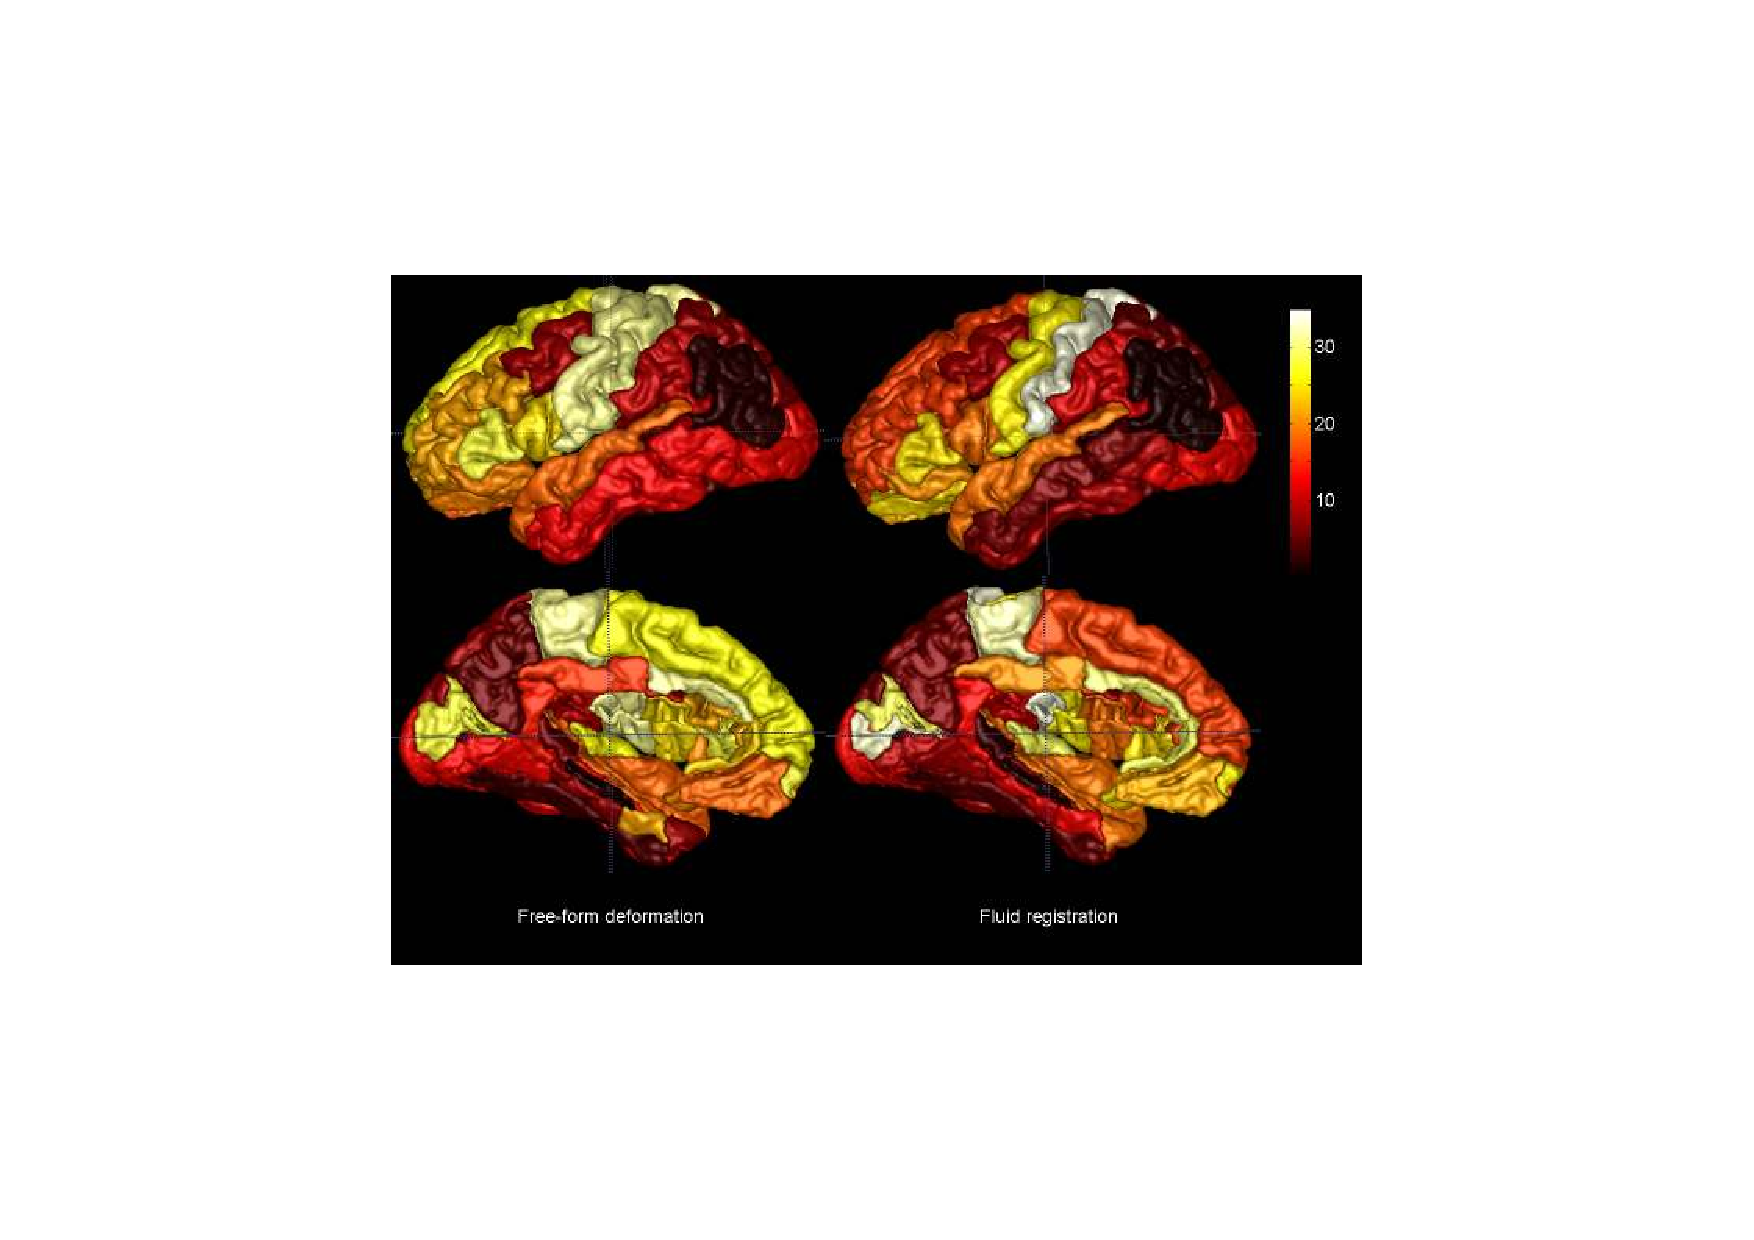
\includegraphics[width=120mm]{figures/ADCompareReg}
\caption{Results of disease progression model for both registration methods (for supplementary methods)}
\label{ADCompareReg}
\end{figure}

\subsection{Disease progression of Huntington's Disease}

\section{Discussion}
In this study, we develop a novel model for disease progression. Our model describes disease progression as a series of events and does not require \emph{a priori} staging of patients. Instead the model provides a 4 dimensional staging framework, in which each patient is ranked along the order of disease events. So far, the detailed classification of AD patients has only been possible post mortem, using the Braak and Braak model. Clinicians have therefore relied on relatively crude clinical tests to classify patients. Our model provides a much more detailed description of disease progression which can be used to classify patients using readily available data (MRI scans). Our results for the disease progression model on MRI data from an fAD and HD cohort confirm previously established patterns of disease progression based on MRI and histological data. 

\note{To DRC: I think we need some more interpretation here. We do see early involvement of memory structures, such as the hippocampus (first and foremost) and other medial temporal lobe structures, but strangely enough not of the entorhinal cortex. What strikes me is the early involvement of the intraparietal cortex, which could overlap with the Default Mode Network. That would be in line with the early involvement of the precuneus that we observe. Another oddball is the early involvement of a frontal region (caudal middle frontal), although this is not entirely consistent when we vary the input of the model.}

Having confirmed the validity of our model, we expect that it will be very useful for diseases for which there are currently no well-established models of disease progression available. Another useful feature of our model is the ease with which other measures, from different brain modalities such as Diffusion Tensor Imaging or functional MRI but also from biochemical and clinical tests can be integrated. This will in the future enable the unification of all these sources of data into a single description of neurological diseases. 

We observe some uncertainty in the average position of each region in our model. This could be caused by the presence of a mixture of disease progression patterns (as discussed below), but we should also acknowledge that the cohort size in both data sets is relatively small. We therefore plan to apply our model to the ADNI [ref] and TrackHD [ref] data sets, which consist of much bigger cohorts. These data sets will allow us to confirm the progression patterns we have established in this study and, more importantly, to further refine them.

Our model depends on correct regional estimates of atrophy. We can distinguish two critical factors in the preprocessing procedures that will affect the atrophy estimates: the correctness of the regional segmentation and the atrophy estimate in itself. We show reasonable robustness with respect to two different methods of non-rigid registration to estimate atrophy. In future studies, we will also explore cortical thickness and automated volume measures in this context. We use the freesurfer parcellation scheme in this study, which subdivides each hemisphere in 35 regions. This is a relatively coarse subdivision, which might explain the fact that we do not observe early involvement of the dorsal anterior cingulate cortex, which was for instance reported by Scahill et al. \note{To DRC: Is this indeed surprising? Are there any other oddballs in the results that need explaining?} The region of compression in that study is however much smaller than the freesurfer segmentation, which might cause the effect in this region to be averaged out. In future work, we will explore finer parcellation schemes.

So far, structural imaging studies have focussed on establishing differences between sub-populations of AD patients that were classified using clinical tests. Scahill et al. for instance subdivide their population of AD and fAD patients into presymptomatic patients and patients with mild and moderate AD. Although this has yielded valuable information about the progress of AD, we argue that our model provides a marker for disease progression that is much more specific with resect to the cellular development of the disease. Our model can be used to rank patients with respect to the typical pattern of disease progression. This could potentially become a powerful tool in clinical trials to investigate whether disease progression slows down in patients in reaction to a treatment.  

Another important issue is the possiblity that disease progression follows two or more progression patterns, rather than the single progression pattern that is assumed in this study. For instance, let us consider the case when there are two patterns of progression present in the data, one in which event A precedes event B and one in which the opposite pattern is present. This will lead to an intermediate probability that event A precedes B which will cause both events to switch position multiple times in the subsequent MCMC procedure. The mean position of both events in the events order will therefore be between the original position values of both events. In future work, we intend to explore a mixture modelling approach to this issue, which will allow us to investigate whether neurological diseases are characterized by one single chain of events, or whether they indeed represent a mixture of progression patterns. This will provide an important further opportunity to subclassify diseases \note{subclassify: weird}. A similar approach has already been developed by Mannilla and co-workers. They study the order of the origination and extinction of species in paleontological data \cite{puolam�ki2006seriation}, using a similar approach as the one developed in this work. In \cite{mannila2000global} they develop a mixture model to study partial orderings in web browsing data, which we could use as a staring point for our mixture modelling approach.

In conclusion, this study presents a novel disease progression model, which subdivdes disease progression into a series of events and which does not rely an previously established staging procedures. We demonstrate our model on cross-sectional MRI data from fAD and HD patients and show broad agreement with existing models of disease progression in these diseases. We are therefore hopeful that this model will find its as a tool to study novel disease progression patterns and as a detailed classification method in fAD and HD.

\bibliographystyle{splncs}
\bibliography{bibliography}

\end{document}


